\documentclass{report}
%%%%%%%%%%%%%% preamble.tex %%%%%%%%%%%%%%
\usepackage[T1]{fontenc}
\usepackage{etoolbox}
% Page Setup
\usepackage[letterpaper, tmargin=2cm, rmargin=0.5in, lmargin=0.5in, bmargin=80pt, footskip=.2in]{geometry}
\usepackage{adjustbox}
\usepackage{graphicx}
\usepackage{tikz}
\usepackage{mathrsfs}
\usepackage{mdframed}

% Create a new toggle
\newtoggle{firstsection}

% Redefine the \chapter command to reset the toggle for each new chapter
\let\oldchapter\chapter
\renewcommand{\chapter}{\toggletrue{firstsection}\oldchapter}

% Redefine the \section command to check the toggle
\let\oldsection\section
\renewcommand{\section}{
    \iftoggle{firstsection}
    {\togglefalse{firstsection}} % If it's the first section, just switch off the toggle for next sections
    {\clearpage} % If it's not the first section, start a new page
    \oldsection
}

% Abstract Design

\usepackage{lipsum}

\renewenvironment{abstract}
 {% Start of environment
  \quotation
  \small
  \noindent
  \rule{\linewidth}{.5pt} % Draw the rule to match the linewidth
  \par\smallskip
  {\centering\bfseries\abstractname\par}\medskip
 }
 {% End of environment
  \par\noindent
  \rule{\linewidth}{.5pt} % Ensure the closing rule also matches
  \endquotation
 }

% Mathematics
\usepackage{amsmath,amsfonts,amsthm,amssymb,mathtools}
\usepackage{xfrac}
\usepackage[makeroom]{cancel}
\usepackage{enumitem}
\usepackage{nameref}
\usepackage{multicol,array}
\usepackage{tikz-cd}
\usepackage{array}
\usepackage{multirow}% http://ctan.org/pkg/multirow
\usepackage{graphicx}

% Colors
\usepackage[dvipsnames]{xcolor}
\definecolor{myg}{RGB}{56, 140, 70}
\definecolor{myb}{RGB}{45, 111, 177}
\definecolor{myr}{RGB}{199, 68, 64}
% Define more colors here...
\definecolor{olive}{HTML}{6B8E23}
\definecolor{orange}{HTML}{CC5500}
\definecolor{brown}{HTML}{8B4513}
% Hyperlinks
\usepackage{bookmark}
\usepackage[colorlinks=true,linkcolor=blue,urlcolor=blue,citecolor=blue,anchorcolor=blue]{hyperref}
\usepackage{xcolor}
\hypersetup{
    colorlinks,
    linkcolor={red!50!black},
    citecolor={blue!50!black},
    urlcolor={blue!80!black}
}

% Text-related
\usepackage{blindtext}
\usepackage{fontsize}
\changefontsize[14]{14}
\setlength{\parindent}{0pt}
\linespread{1.2}

% Theorems and Definitions
\usepackage{amsthm}
\renewcommand\qedsymbol{$\blacksquare$}

% Define a new theorem style
\newtheoremstyle{mytheoremstyle}% name
  {}% Space above
  {}% Space below
  {}% Body font
  {}% Indent amount
  {\bfseries}% Theorem head font
  {.}% Punctuation after theorem head
  {.5em}% Space after theorem head
  {}% Theorem head spec (can be left empty, meaning ‘normal’)

% Apply the new theorem style to theorem-like environments
\theoremstyle{mytheoremstyle}

\newtheorem{theorem}{Theorem}[section]  
\newtheorem{definition}[theorem]{Definition} 
\newtheorem{lemma}[theorem]{Lemma}  
\newtheorem{corollary}[theorem]{Corollary}
\newtheorem{axiom}[theorem]{Axiom}
\newtheorem{example}[theorem]{Example}
\newtheorem{equiv_def}[theorem]{Equivalent Definition}

% tcolorbox Setup
\usepackage[most,many,breakable]{tcolorbox}
\tcbuselibrary{theorems}

% Define custom tcolorbox environments here...

%================================
% EXAMPLE BOX
%================================
% After you have defined the style and other theorem environments
\definecolor{myexamplebg}{RGB}{245, 245, 245} % Very light grey for background
\definecolor{myexamplefr}{RGB}{120, 120, 120} % Medium grey for frame
\definecolor{myexampleti}{RGB}{60, 60, 60}    % Darker grey for title

\newtcbtheorem[]{Example}{Example}{
    colback=myexamplebg,
    breakable,
    colframe=myexamplefr,
    coltitle=myexampleti,
    boxrule=1pt,
    sharp corners,
    detach title,
    before upper=\tcbtitle\par\vspace{-20pt}, % Reduced the space after the title
    fonttitle=\bfseries,
    description font=\mdseries,
    separator sign none,
    description delimiters={}{}, % No delimiters around the title
}{ex}
%================================
% Solution BOX
%================================
\makeatletter
\newtcolorbox{solution}{enhanced,
	breakable,
	colback=white,
	colframe=myg!80!black,
	attach boxed title to top left={yshift*=-\tcboxedtitleheight},
	title=Solution,
	boxed title size=title,
	boxed title style={%
			sharp corners,
			rounded corners=northwest,
			colback=tcbcolframe,
			boxrule=0pt,
		},
	underlay boxed title={%
			\path[fill=tcbcolframe] (title.south west)--(title.south east)
			to[out=0, in=180] ([xshift=5mm]title.east)--
			(title.center-|frame.east)
			[rounded corners=\kvtcb@arc] |-
			(frame.north) -| cycle;
		},
}
\makeatother

% %================================
% % Question BOX
% %================================
\makeatletter
\newtcbtheorem{question}{Question}{enhanced,
	breakable,
	colback=white,
	colframe=myb!80!black,
	attach boxed title to top left={yshift*=-\tcboxedtitleheight},
	fonttitle=\bfseries,
	title={#2},
	boxed title size=title,
	boxed title style={%
			sharp corners,
			rounded corners=northwest,
			colback=tcbcolframe,
			boxrule=0pt,
		},
	underlay boxed title={%
			\path[fill=tcbcolframe] (title.south west)--(title.south east)
			to[out=0, in=180] ([xshift=5mm]title.east)--
			(title.center-|frame.east)
			[rounded corners=\kvtcb@arc] |-
			(frame.north) -| cycle;
		},
	#1
}{question}
\makeatother

%%%%%%%%%%%%%%%%%%%%%%%%%%%%%%%%%%%%%%%%%%%
% TABLE OF CONTENTS
%%%%%%%%%%%%%%%%%%%%%%%%%%%%%%%%%%%%%%%%%%%


\usepackage{tikz}
\definecolor{doc}{RGB}{0,60,110}
\usepackage{titletoc}
\contentsmargin{0cm}
\titlecontents{chapter}[14pc]
{\addvspace{30pt}%
	\begin{tikzpicture}[remember picture, overlay]%
		\draw[fill=doc!60,draw=doc!60] (-7,-.1) rectangle (-0.9,.5);%
		\pgftext[left,x=-5.5cm,y=0.2cm]{\color{white}\Large\sc\bfseries Chapter\ \thecontentslabel};%
	\end{tikzpicture}\color{doc!60}\large\sc\bfseries}%
{}
{}
{\;\titlerule\;\large\sc\bfseries Page \thecontentspage
	\begin{tikzpicture}[remember picture, overlay]
		\draw[fill=doc!60,draw=doc!60] (2pt,0) rectangle (4,0.1pt);
	\end{tikzpicture}}%
\titlecontents{section}[3.7pc]
{\addvspace{2pt}}
{\contentslabel[\thecontentslabel]{3pc}}
{}
{\hfill\small \thecontentspage}
[]
\titlecontents*{subsection}[3.7pc]
{\addvspace{-1pt}\small}
{}
{}
{\ --- \small\thecontentspage}
[ \textbullet\ ][]

\makeatletter
\renewcommand{\tableofcontents}{
	\chapter*{%
	  \vspace*{-20\p@}%
	  \begin{tikzpicture}[remember picture, overlay]%
		  \pgftext[right,x=15cm,y=0.2cm]{\color{doc!60}\Huge\sc\bfseries \contentsname};%
		  \draw[fill=doc!60,draw=doc!60] (13,-.75) rectangle (20,1);%
		  \clip (13,-.75) rectangle (20,1);
		  \pgftext[right,x=15cm,y=0.2cm]{\color{white}\Huge\sc\bfseries \contentsname};%
	  \end{tikzpicture}}%
	\@starttoc{toc}}
\makeatother

\newcommand{\liff}{\llap{$\iff$}}
\newcommand{\rap}[1]{\rrap{\text{ (#1)}}}
\newcommand{\red}[1]{\textcolor{red}{#1}}
\newcommand{\blue}[1]{\textcolor{blue}{#1}}
\newcommand{\vi}[1]{\textcolor{violet}{#1}}
\newcommand{\olive}[1]{\textcolor{olive}{#1}}
\newcommand{\teal}[1]{\textcolor{teal}{#1}}
\newcommand{\brown}[1]{\textcolor{brown}{#1}}
\newcommand{\orange}[1]{\textcolor{orange}{#1}}
\newcommand{\tCaC}{\text{ \CaC }}
\newcommand{\CaC}{\red{CaC} }
\newcommand{\As}[1]{Assume \red{#1}}
\newcommand{\vdone}{\vi{\text{ (done) }}}
\newcommand{\bdone}{\blue{\text{ (done) }}}
\newcommand{\tdone}{\teal{\text{ (done) }}}
\newcommand{\odone}{\olive{\text{ (done) }}}
\newcommand{\bodone}{\brown{\text{ (done) }}}
\newcommand{\ordone}{\orange{\text{ (done) }}}
\newcommand{\ld}{\lambda}
\newcommand{\vecta}[1]{\textbf{#1}}
\newcommand{\set}[1]{\left\{ #1 \right\}}
\newcommand{\bset}[1]{\Big\{ #1 \Big\}}
\newcommand{\inR}{\in\R}
\newcommand{\inn}{\in\N}
\newcommand{\inz}{\in\Z}
\newcommand{\inr}{\in\R}
\newcommand{\inc}{\in\C}
\newcommand{\inq}{\in\Q}
\newcommand{\norm}[1]{\| #1 \|}
\newcommand{\bnorm}[1]{\Big\| #1 \Big\|}
\newcommand{\gen}[1]{\langle #1 \rangle}
\newcommand{\abso}[1]{\left|#1\right|}
\newcommand{\myref}[2]{\hyperref[#2]{#1\ \ref*{#2}}}
\newcommand{\customref}[2]{\hyperref[#1]{#2}}
\newcommand{\power}[1]{\mathcal{P}(#1)}
\newcommand{\dcup}{\mathbin{\dot{\cup}}}
\newcommand{\diam}[1]{\text{diam}\, #1}
\newcommand{\at}{\Big|}
\newcommand{\quotient}{\diagup}
\let\originalphi\phi % Store the original \phi in \originalphi
\renewcommand{\phi}{\varphi} % Redefine \phi to \varphi
\newcommand{\pfi}{\originalphi} % Define \pfi to display the original \phi
\newcommand{\diota}{\dot{\iota}}
\newcommand{\Log}{\operatorname{Log}}
\newcommand{\id}{\text{\textbf{id}}}
\usepackage{amsmath}

\makeatletter
\NewDocumentCommand{\extp}{e{^}}{%
  \mathop{\mathpalette\extp@{#1}}\nolimits
}
\NewDocumentCommand{\extp@}{mm}{%
  \bigwedge\nolimits\IfValueT{#2}{^{\extp@@{#1}#2}}%
  \IfValueT{#1}{\kern-2\scriptspace\nonscript\kern2\scriptspace}%
}
\newcommand{\extp@@}[1]{%
  \mkern
    \ifx#1\displaystyle-1.8\else
    \ifx#1\textstyle-1\else
    \ifx#1\scriptstyle-1\else
    -0.5\fi\fi\fi
  \thinmuskip
}
\makeatletter
\usepackage{pifont}
\makeatletter
\newcommand\Pimathsymbol[3][\mathord]{%
  #1{\@Pimathsymbol{#2}{#3}}}
\def\@Pimathsymbol#1#2{\mathchoice
  {\@Pim@thsymbol{#1}{#2}\tf@size}
  {\@Pim@thsymbol{#1}{#2}\tf@size}
  {\@Pim@thsymbol{#1}{#2}\sf@size}
  {\@Pim@thsymbol{#1}{#2}\ssf@size}}
\def\@Pim@thsymbol#1#2#3{%
  \mbox{\fontsize{#3}{#3}\Pisymbol{#1}{#2}}}
\makeatother
% the next two lines are needed to avoid LaTeX substituting upright from another font
\input{utxmia.fd}
\DeclareFontShape{U}{txmia}{m}{n}{<->ssub * txmia/m/it}{}
% you may also want
\DeclareFontShape{U}{txmia}{bx}{n}{<->ssub * txmia/bx/it}{}
% just in case
%\DeclareFontShape{U}{txmia}{l}{n}{<->ssub * txmia/l/it}{}
%\DeclareFontShape{U}{txmia}{b}{n}{<->ssub * txmia/b/it}{}
% plus info from Alan Munn at https://tex.stackexchange.com/questions/290165/how-do-i-get-a-nicer-lambda?noredirect=1#comment702120_290165
\newcommand{\pilambdaup}{\Pimathsymbol[\mathord]{txmia}{21}}
\renewcommand{\lambda}{\pilambdaup}
\renewcommand{\tilde}{\widetilde}
\DeclareMathOperator*{\esssup}{ess\,sup}
\newcommand{\bluecheck}{}%
\DeclareRobustCommand{\bluecheck}{%
  \tikz\fill[scale=0.4, color=blue]
  (0,.35) -- (.25,0) -- (1,.7) -- (.25,.15) -- cycle;%
}


\usepackage{tikz}
\newcommand*{\DashedArrow}[1][]{\mathbin{\tikz [baseline=-0.25ex,-latex, dashed,#1] \draw [#1] (0pt,0.5ex) -- (1.3em,0.5ex);}}

\newcommand{\C}{\mathbb{C}}	
\newcommand{\F}{\mathbb{F}}
\newcommand{\N}{\mathbb{N}}
\newcommand{\Q}{\mathbb{Q}}
\newcommand{\R}{\mathbb{R}}
\newcommand{\Z}{\mathbb{Z}}



\title{Notes on Linear Algebra}
\author{Eric Liu}
\date{}
\begin{document}
\maketitle
\newpage% or \cleardoublepage
% \pdfbookmark[<level>]{<title>}{<dest>}
\pdfbookmark[section]{\contentsname}{toc}

\tableofcontents
\pagebreak
\chapter{Linear Algebra Done Outrageous}
\section{Determinant}
\begin{mdframed}
Let $N\triangleq \set{1,\dots,n}$. Given a permutation $\sigma \in S_n$, if  
\begin{align*}
\bset{(x,y)\in N^2:x<y\text{ and }\sigma(x)>\sigma (y)}\text{ has even numbers of element. }
\end{align*}
We say $\sigma$ is \textbf{even} and write
\begin{align*}
\operatorname{sgn}\sigma=1
\end{align*}
Given some $n$-by-$n$ square matrix $A$, its determinant is by definition 
\begin{align*}
\operatorname{det}A\triangleq  \sum_{\sigma \in S_n} \Big(\operatorname{sgn}\sigma \prod_{k=1}^n  A_{\sigma (k),k} \Big)
\end{align*}
Or equivalently, the unique alternating multilinear map from $(\F^n)^n$ to $\F$ such that 
 \begin{align*}
\operatorname{det}(I)=1
\end{align*}

\end{mdframed}
\begin{theorem}
\label{Det}
\textbf{(Determinant)} Let $\set{v_1,\dots ,v_n}$ be a basis for $V$ and  $\set{\omega_1,\dots ,\omega_n}$ be its dual basis. We have
\begin{align*}
\operatorname{sgn}\sigma = \operatorname{det}\Big(\begin{bmatrix}
    \omega_1 v_{\sigma (1)} & \cdots & \omega_1 v_{\sigma (n)}\\
    \vdots & \ddots & \vdots \\
    \omega_n v_{\sigma (1)} & \cdots & \omega_n v_{\sigma (n)}  
\end{bmatrix} \Big) 
\end{align*}
\end{theorem}
\section{Dual Space}
\begin{mdframed}
Given a vector space $V$ over  $\R$, the map  $\alpha :U\rightarrow (U^\vee)^{\vee}$ defined by 
\begin{align*}
\alpha (x)(\rho)\triangleq \rho (x)
\end{align*}
is a vector space isomorphism. Given a linear map $A:V\rightarrow W$, we may define its \textbf{dual map} $A^\vee:W^{\vee}\rightarrow V^{\vee}$ by 
\begin{align*}
A^{\vee}(\xi)(v)\triangleq \xi \circ A(v) 
\end{align*}
\end{mdframed}
\section{Tensor Algebra}
\begin{abstract}
In this section, by the term \textbf{ring}, we mean a ring with a multiplication identity, and by the term \textbf{real algebra}, we mean a real vector space equipped with a vector multiplication compatible with both scalar multiplication and addition. In this definition, for a real algebra $A$ to be a ring, $A$ must be associative.  By the term \textbf{ideal}, we mean a 2-sided ideal. If we say a multi-linear map $M:V^k\rightarrow Z$ is \textbf{alternating}, we mean that $M$ maps $(v_1,\dots ,v_n)$ to $0$ if two arguments coincide.
\end{abstract}
\begin{mdframed}
Given a finite collection $(V_1,\dots ,V_n)$ of finite dimensional real vector space, by the term \textbf{tensor product of $V_1,\dots ,V_n$}, we mean a real vector space  usually denoted by $V_1 \otimes \cdots \otimes  V_n$ and a multilinear map  $\otimes  : V_1 \times \cdots \times V_n \rightarrow V_1 \otimes  \cdots \otimes  V_n$ satisfying the universal property: If $B:V_1 \times \cdots \times V_n\rightarrow Z$ is a multilinear map, then there exists a unique linear map $\beta :V_1\otimes \cdots \otimes  V_n$ such that 
\begin{align*}
B(v_1,\dots ,v_n)=\beta (v_1\otimes \cdots \otimes  v_n)
\end{align*}
In other words, we have the commutative diagram
% https://q.uiver.app/#q=WzAsMyxbMCwwLCJWXFx0aW1lcyBXIl0sWzAsMiwiViBcXG90aW1lcyBXIl0sWzIsMCwiVSJdLFswLDIsIkIiXSxbMSwyLCJcXGV4aXN0cyEgXFxiZXRhIiwyLHsic3R5bGUiOnsiYm9keSI6eyJuYW1lIjoiZGFzaGVkIn19fV0sWzAsMSwiKHYsdylcXG1hcHN0byB2XFxvdGltZXMgdyIsMl1d
\[\begin{tikzcd}
	{V_1\times \cdots \times V_n} && U \\
	\\
	{V_1 \otimes \cdots \otimes   V_n}
	\arrow["B", from=1-1, to=1-3] 
	\arrow["{\otimes }"', from=1-1, to=3-1]
	\arrow["{\exists! \beta}"', dashed, from=3-1, to=1-3]
\end{tikzcd}\]
This approach indeed define a pair of vector space and multilinear map uniquely up to isomorphism, in the sense of \myref{Theorem}{UoT}, where we define the isomorphism between tensor product. 
\end{mdframed}
\begin{theorem}
\label{UoT}
\textbf{(Uniqueness of Tensor product)} Given a finite collection $(V_1,\dots, V_n)$ of finite dimensional real vector space, if $V_1 \otimes \cdots \otimes  V_n ,V_1\otimes  '\cdots \otimes  ' V_n$ both satisfy the universal property, then there exists an linear isomorphism $T:V_1 \otimes  \cdots \otimes  V_n \rightarrow V_1 \otimes' \cdots \otimes  ' V_n $ such that 
\begin{align*}
T(v_1\otimes  \cdots \otimes  v_n)=v_1 \otimes  '\cdots \otimes  'v_n
\end{align*}
\end{theorem}
\begin{proof}
Because $V_1 \otimes  \cdots \otimes  V_n$ satisfies the universal property, there exists a linear map $T:V_1 \otimes  \cdots \otimes  V_n\rightarrow V_1 \otimes'  \cdots \otimes' V_n  $ such that  
\begin{align*}
\otimes' =T \circ \otimes  
\end{align*}
It remains to show $T$ is bijective. Similarly, because $V_1 \otimes ' \cdots \otimes'  V_n$ satisfies the universal property, there exists a linear map $T':V_1 \otimes'  \cdots \otimes'  V_n\rightarrow V_1 \otimes  \cdots \otimes V_n  $ such that 
\begin{align*}
\otimes = T' \circ \otimes  '
\end{align*}
Composing the two equations, we have 
\begin{align*}
\otimes '=T\circ T' \circ \otimes  '
\end{align*}
It then follows from uniqueness of the induced linear map in universal property that $T \circ T'=\textbf{id}:V_1 \otimes  ' \cdots \otimes  'V_n \rightarrow V_1 \otimes  ' \cdots \otimes  'V_n$. This implies $T$ is indeed bijective. 
\end{proof}
\begin{mdframed}
We have shown that tensor products is unique up to isomorphism. A construction further shows that if $B_i$ are bases for $V_i$, then 
 \begin{align*}
\set{v_1 \otimes  \cdots \otimes v_n: v_i \in B_i\text{ for all }1\leq i\leq n  }\text{ form a basis for }V_1 \otimes  \cdots \otimes  V_n
\end{align*}
\end{mdframed}
\begin{theorem}
\textbf{(Associativity of the Tensor product)} Given three finite-dimensional real vector spaces $X,Y,Z$,  there exists a unique linear isomorphism $F:X\otimes  Y\otimes  Z\rightarrow (X\otimes  Y)\otimes  Z$ that satisfy 
\begin{align*}
F(x\otimes  y \otimes  z)=(x\otimes  y)\otimes  z
\end{align*}
\end{theorem}
\begin{proof}
Define $f:X\times Y \times Z\rightarrow (X\otimes  Y)\otimes Z$ by 
\begin{align*}
f(x,y,z)\triangleq (x \otimes  y)\otimes z
\end{align*}
It follows from the universal property that there exists a unique linear map $F:X\otimes  Y\otimes Z\rightarrow (X \otimes  Y)\otimes  Z $ such that 
\begin{align*}
F(x\otimes  y\otimes  z)=f(x,y,z)= (x \otimes y) \otimes z 
\end{align*}
It remains to show \vi{$F$ is bijective}.  For all $z\in Z$, define $h_z:X\times Y\rightarrow X \otimes  Y\otimes Z$ by 
\begin{align*}
h_z(x,y)\triangleq x\otimes  y\otimes  z
\end{align*}
If follows from the universal property that there exists a unique linear map $H_z:X\otimes  Y \rightarrow X \otimes  Y\otimes  Z$ such that 
\begin{align*}
H_z(x \otimes  y)=h_z(x,y)=x \otimes  y \otimes  z
\end{align*}
Define $h:(X\otimes  Y)\times Z\rightarrow X\otimes Y \otimes Z$ by 
\begin{align*}
h(v,z)\triangleq H_z(v)
\end{align*}
It is clear that $h$ in linear in  $(X\otimes  Y)$. We now show $h$ is linear in  $Z$, that is 
 \begin{align*}
   \olive{H_{c_1z_1+z_2}=c_1H_{z_1}+H_{z_2}}
\end{align*}
By definition, 
\begin{align*}
  (c_1H_{z_1}+H_{z_2})(x\otimes  y)&=c_1 x\otimes  y\otimes  z_1+ x\otimes  y \otimes  z_2\\
  &= x\otimes  y\otimes  (c_1z_1+z_2)=h_{c_1z_1+z_2}(x,y)
\end{align*}
It then follows from the uniqueness part of the universal property that $H_{c_1z_1+z_2}=c_1H_{z_1}+H_{z_2}$. $\odone$  \\


We have shown $h$ is indeed bilinear. It follows from the universal property that there exists a unique linear map $H:(X\otimes  Y)\otimes  Z\rightarrow X\otimes Y\otimes Z$ such that 
\begin{align*}
H((x\otimes y)\otimes z)=h(x\otimes  y,z)=H_z(x\otimes  y)=x\otimes  y\otimes  z
\end{align*}
Let $\otimes:X\times Y\times Z\rightarrow X\otimes  Y\otimes  Z$ denotes the tensor product, we now have 
\begin{align*}
\otimes = H \circ F \circ \otimes 
\end{align*}
It then follows from universal property that $H \circ F=\textbf{id}:X\otimes  Y\otimes  Z\rightarrow X\otimes  Y\otimes  Z$. This implies $F$ is indeed bijective. $\vdone$
\end{proof}
\begin{mdframed}
Let $V$ be a finite-dimensional real vector space. By its  \textbf{tensor algebra}, we mean any real associative algebra $T(V)$ with an injective linear map $\diota:V\rightarrow T(V)$ that satisfies the universal property: If $A$ is a real associative algebra and $f:V\rightarrow A$ is a linear map, then there exists a unique algebra homomorphism $F:T(V)\rightarrow A$ such that the diagram  
% https://q.uiver.app/#q=WzAsMyxbMiwwLCJUKFYpIl0sWzIsMiwiQSJdLFswLDAsIlYiXSxbMiwwLCJcXGRvdHtcXGlvdGF9Il0sWzIsMSwiZiIsMl0sWzAsMSwiRiIsMCx7InN0eWxlIjp7ImJvZHkiOnsibmFtZSI6ImRhc2hlZCJ9fX1dXQ==
\[\begin{tikzcd}
	V && {T(V)} \\
	\\
	&& A
	\arrow["{\dot{\iota}}", from=1-1, to=1-3]
	\arrow["f"', from=1-1, to=3-3]
	\arrow["F", dashed, from=1-3, to=3-3]
\end{tikzcd}\]
commutes. The proof that such definition is indeed unique up to isomorphism is similar to that of \myref{Theorem}{UoT} and thus omitted. We now give the most useful construction. \\

Let $V$ be finite-dimensional real vector space. We use the notation 
 \begin{align*}
T^n(V)\triangleq  \overbrace{V \otimes  \cdots \otimes  V}^{n\text{ copies }}
\end{align*}
and call $T^{n}(V)$ the \textbf{$n$-th tensor power of $V$} or the \textbf{$n$-fold tensor product of  $V$}. Define  
\begin{align*}
  T(V)&\triangleq  \bigoplus_{n=0}^{\infty} T^n(V)\\
  &=\R \oplus V \oplus (V\otimes V) \oplus (V\otimes V \otimes V)  \oplus \cdots 
\end{align*}
and define for all $f,g \in T(V)$ the multiplication 
\begin{align*}
  (fg)(n)\triangleq   \sum_{k=0}^{n}f(k)g(n-k)
\end{align*}
where 
\begin{align*}
  &\Big(\sum_{I} a_I v_{I(1)}\otimes \cdots \otimes  v_{I(k)}\Big)\Big(\sum_J b_J v_{J(1)}\otimes  \cdots \otimes  v_{J(l)}\Big)\\
  &\triangleq \sum_{I,J} a_I b_J v_{I(1)}\otimes \cdots \otimes  v_{I(k)}\otimes  v_{J(1)}\otimes  \cdots \otimes  v_{J(l)}
\end{align*}
where $\set{v_1,\dots ,v_m}$ is some basis for $V$, $I$ run through the set of function that maps $\set{1,\dots ,k}$ into $\set{1,\dots ,m}$ and $J$ run through the set of function that maps  $\set{1,\dots ,l}$ into $\set{1,\dots ,m}$. For example, given two elements  
\begin{align*}
  (5,0,v_1\otimes v_2,0,0,\dots )\text{ and }(7,v_3,0,0,\dots)
\end{align*}
of $T(V)$, their product is defined to be 
\begin{align*}
  (35,5v_3,7v_1\otimes v_2, v_1 \otimes v_2 \otimes v_3 ,0,0,\dots)
\end{align*}
Tedious effort shows that our multiplication is consistent with abuse of notation in the sense that if $f,g\in T(V)$ is defined by  
\begin{align*}
 f(k)\triangleq \begin{cases}
   w_1\otimes \cdots \otimes  w_n & \text{ if $k=n$ }\\
   0& \text{ if otherwise }
 \end{cases} \text{ and } g(k)\triangleq \begin{cases}
   w_{n+1}\otimes  \cdots \otimes  w_{n+l}& \text{ if $k=l$ }\\
   0& \text{ if otherwise }
 \end{cases} 
\end{align*}
then 
\begin{align*}
  (fg)(k)=\begin{cases}
    w_1\otimes  \cdots \otimes  w_{n+l}& \text{ if $n=k+l$ }\\
    0& \text{ if otherwise }
  \end{cases}
\end{align*}


does form an associative algebra with multiplication identity $1\inr$. Thus, $T(V)$ is in fact a ring. Let $I(V)\subseteq T(V)$ be the ideal generated by $\set{v\otimes v:v \in V}$. By definition, ideal $I(V)$ is a subgroup of $T(V)$. To see that $I(V)$ is closed under scalar multiplication, observe that for all $t\inr\text{ and }x\in T(V)$, the scalar multiplication $tx$ is identical to $tx$ where $t$ is treated as an element of $T(V)$, so it follows from definition of ideal that $I(V)$ is also a vector subspace of $T(V)$. Let $\set{v_1,\dots ,v_n}$ be a basis for $V$, and let  $S$ be the set of function that maps  $\set{1,\dots ,n}$ into $\set{1,\dots ,k}$. We know for a fact that 
\begin{align*}
T^k(V) = \operatorname{span} \set{v_{I(1)}\otimes  \cdots \otimes  v_{I(k)}: I \in S}
\end{align*}
If we define $I^k(V)\triangleq I(V)\cap T^k(V)$, one then have 
\begin{align}
\label{ikv} I^k(V)=\operatorname{span}\set{v_{I(1)}\otimes \cdots \otimes  v_{I(k)}:I(j)=I(j+1)\text{ for some }j}
\end{align}
This is proved by showing $I^0(V)\oplus  I^1(V)\oplus  I^2(V)\oplus  \cdots $ is indeed the smallest ideal containing $\set{v\otimes  v:v \in V}$. Define an equivalence class on $T(V)$ by 
\begin{align*}
x\sim  y\overset{\triangle}{\iff }x-y \in I (V)
\end{align*}
Because ideal form a subgroup, we see that our definition indeed give an equivalence relation. We then can define on the set of equivalence class $T(V)\setminus I(V)$ addition, scalar multiplication and vector multiplication 
\begin{align*}
[x]+[y]\triangleq [x+y] \text{ and }[x]\wedge [y]\triangleq [xy]\text{ and }c[x]\triangleq [cx]
\end{align*}
which is well defined and form an algebra as one can check. We call this algebra $T(V)\setminus I(V)$ the \textbf{exterior algebra} $\wedge ^* (V)$. Note that if we refer to $v,w \in T^k(V)$ as elements of $\wedge ^*(V) $, we mean $[v],[w]$. Immediately, we see that the wedge product is \textbf{alternating} in the sense that if $v\in V$, then 
\begin{align*}
v\wedge v=0 
\end{align*}
and is \textbf{anti-symmetric} in the sense that if $v,w \in V$, then 
\begin{align*}
v\wedge w= -w\wedge  v
\end{align*}
We use the notation 
\begin{align*}
\wedge^k(V) \triangleq \bset{ [x] \in \wedge ^*(V): x \in \overbrace{V \otimes  \cdots \otimes  V}^{k\text{ copies }}} 
\end{align*}
Immediately from \myref{Equation}{ikv}, we see that $\wedge ^k (V) $ is the vector space 
\begin{align*}
\operatorname{span}\set{v_{I(1)}\wedge  \cdots \wedge  v_{I(k)}:I \in S  }
\end{align*}
where $\set{v_1,\dots ,v_n}$ is a basis for $V$ and $S$ is the set of function that maps  $\set{1,\dots ,k}$ into $\set{1,\dots ,n}$. If we define the vector subspace $I^k(V)\triangleq T^k(V)\cap I(V)$, there exists a natural vector space isomorphism
\begin{align*}
\wedge  ^k(V)\underset{\text{ v.s. }}{\cong }T^k(V)\setminus I^k(V);[x]\leftrightarrow [x]
\end{align*}
where $T^k(V)\setminus I^k(V)$ is the quotient vector space.
\end{mdframed}
\begin{theorem}
\label{Universal mapping property for alternating $k$-linear map}
\textbf{(Universal mapping property for alternating $k$-linear map)} For any vector space $Z$ over  $\R$ and any alternating  $k$-linear map  $f:V^k\rightarrow Z$, there is a unique linear map $F:\bigwedge ^k V\rightarrow Z $ such that the diagram 
% https://q.uiver.app/#q=WzAsMyxbMCwwLCJcXGJpZ3dlZGdlXmsgViAiXSxbMCwyLCJWXmsiXSxbMiwyLCJaIl0sWzEsMCwiXFx3ZWRnZSAiXSxbMCwyLCJcXHRpbGRle2Z9Il0sWzEsMiwiZiIsMl1d
\[\begin{tikzcd}
	{\bigwedge^k V } \\
	\\
	{V^k} && Z
	\arrow["F", from=1-1, to=3-3]
	\arrow["{\wedge }", from=3-1, to=1-1]
	\arrow["f"', from=3-1, to=3-3]
\end{tikzcd}\]
commute, i.e., 
\begin{align*}
F(v_1\wedge \cdots \wedge  v_k  )=f(v_1,\dots ,v_k) \text{ for all }v_1,\dots,v_k \in V
\end{align*}
\end{theorem}
\begin{proof}
By \customref{Universal Property of Tensor Product}{universal property of tensor product}, there exists unique linear map $h:T^k(V)\rightarrow Z$ such that 
 \begin{align*}
h(v_1 \otimes  \cdots \otimes  v_k)=f(v_1,\cdots ,v_k)
\end{align*}
Because $f$ is alternating, we see from the characterization of $I^k(V)$ given in \myref{Equation}{ikv} that $h$ vanishes on $I^k(V)$. We then can induce a linear map 
\begin{align*}
F:\wedge^k (V)\cong \frac{T^k(V)}{I^k(V)} \rightarrow Z 
\end{align*}
by $F([x])\triangleq h(x)$. This then give us the desired  
\begin{align*}
F(v_1 \wedge  \cdots \wedge  v_k )=h(v_1\otimes  \cdots \otimes  v_k)=f(v_1,\dots ,v_k)
\end{align*}
Note that $F$ is unique because all such linear map take the same values on  $\set{v_{I(1)}\wedge  \cdots \wedge  v_{I(k)}:I \in S }$ which spans $\wedge ^k(V) $. 
\end{proof}
\begin{mdframed}
Let $\set{w_1,\dots ,w_l}\subseteq V$ be linear independent. An immediate consequence of the \customref{Universal mapping property for alternating $k$-linear map}{universal mapping property for alternating $k$-linear map} is that one may define alternating multilinear $f:V^l\rightarrow \R$ by 
\begin{align*}
B(v_1,\dots ,v_l)\triangleq \operatorname{det}(M)\text{ where }v_i= \sum_j M_{i,j}w_j
\end{align*}
and see that $F:\wedge^l (V)\rightarrow \R $ take $w_1\wedge  \cdots \wedge  w_l$ to $1$. This implies that  
\begin{align*}
w_1\wedge  \cdots \wedge  w_l \neq 0  
\end{align*}
\end{mdframed}
\begin{theorem}
\label{ASo}
\textbf{(Anti-symmetry of wedge product)} If $\alpha \in \wedge ^k (V),\beta \in \wedge ^l (V)  $, then $\alpha \wedge  \beta =(-1)^{kl}(\beta  \wedge  \alpha  )  $. 
\end{theorem}
\begin{proof}
Let $v_1,\dots ,v_n$ be a basis of $V$. Let $S_k$ be the space of function that maps $\set{1,\dots ,k}$into  $\set{1,\dots,n}$ , $S_l$ be the space of function that maps  $\set{1,\dots ,l}$ into  $\set{1,\dots ,n}$. We may then write 
\begin{align*}
\alpha = \sum_{I \in S_k} a_I (v_{I(1)}\wedge \cdots \wedge  v_{I(k)})\text{ and }\beta =\sum_{J \in S_l} b_J (v_{J(1)}\wedge \cdots \wedge v_{J(l)}  )
\end{align*}
and compute 
\begin{align*}
\alpha \wedge \beta &= \sum_{I \in S_k,J\in S_l}a_Ib_J (v_{I(1)}\wedge \cdots \wedge v_{I(k)} \wedge  v_{J(1)} \wedge \cdots  \wedge v_{J(l)}   )\\
&=   \sum_{I \in S_k,J\in S_l}(-1)a_Ib_J (v_{I(1)}\wedge \cdots \wedge   v_{J(1)} \wedge  v_{I(k)}\cdots\wedge \cdots  \wedge v_{J(l)}   )   \\
&=  \sum_{I \in S_k,J\in S_l}(-1)^ka_Ib_J (v_{J(1)}\wedge v_{I(1)}\wedge  \cdots \wedge    v_{I(k)} \wedge  v_{J(2)} \wedge \cdots  \wedge v_{J(l)}   )   \\
  &=\sum_{I \in S_k,J\in S_l}(-1)^{kl}a_Ib_J (v_{J(1)}\wedge \cdots \wedge  v_{J(l)}\wedge v_{I(1)} \wedge   \cdots \wedge   v_{I(k)})= (-1)^{kl}\beta \wedge  \alpha  
\end{align*}
\end{proof}
\begin{mdframed}
Following from \myref{Theorem}{ASo}, \myref{Equation}{ikv} and tedious effort, one can see that if $\set{v_1,\dots ,v_n}$ is a basis for $V$, then 
 \begin{align*}
\set{v_{i_1}\wedge  \cdots \wedge  v_{i_k}:1\leq i_1< \cdots < i_k\leq n  }
\end{align*}
form a basis for $\wedge^k(V)$. If $A:V\rightarrow W$ is a linear map, we define linear map $\wedge^k A:\wedge^k (V)\rightarrow \wedge^k (W) $ by linear extension of 
\begin{align*}
\wedge^k(A)(v_1\wedge  \cdots \wedge   v_n)=Av_1 \wedge  \cdots \wedge  Av_n  
\end{align*}
Note that if  $A:V\rightarrow V$ and $\operatorname{dim}(V)=n$, then $\wedge ^nA: \wedge^n (V)\rightarrow \wedge ^n(V)$ is given by the determinant since given basis  $\set{v_1,\dots ,v_n}$, we have 
\begin{align*}
\wedge^nA(v_1 \wedge  \cdots \wedge  v_n   )&=\Big(\sum_j A_{j,1}v_j\Big)\wedge  \cdots \wedge \Big(\sum_j A_{j,n}v_j\Big)    \\
&=\sum_{\sigma \in S_n} A_{\sigma (1),1}\cdots A_{\sigma (n),n}v_{\sigma (1)}\wedge  \cdots \wedge  v_{\sigma(n)}   \\
&=\sum_{\sigma \in S_n}\operatorname{sgn}(\sigma)A_{\sigma(1),1}\cdots A_{\sigma(n),n}v_1\wedge  \cdots \wedge  v_n
\end{align*}
\end{mdframed}
\section{Norm and Inner Product}
\begin{mdframed}
This section contains
\begin{enumerate}[label=(\alph*)]
  \item definition and basic properties of the term \textbf{norm}
  \item definition and basic properties of the term \textbf{inner product}
  \item definition and basic properties of the term \textbf{positive semi-definite Hermitian form}
  \item full statement and proof of \textbf{Cauchy Schwarz Inequality} for both inner product space and positive semi-definite Hermitian form  
  \item statement and proof of \textbf{SVD} (singular value decomposition). 
\end{enumerate}
\end{mdframed}
\textbf{(Norm Axiom Part)}
\begin{mdframed}
Recall that by a \textbf{normed space} $V$, we mean a vector space over a sub-field $\F$ of $\C$ equipped with  $\norm{\cdot}:V\to \R_0^+$ satisfying the following $\underline{\text{axioms}}$: 
\begin{enumerate}[label=(\alph*)]
  \item $\norm{x}=0 \implies x=0$ (positive-definiteness)
  \item $\norm{sx}=\abso{s}\cdot \norm{x}$ for all $s \in \F$ and $x\in V$ (absolute-homogenity)
  \item $\norm{x+y}\leq \norm{x}+\norm{y}$ for all $x,y \in V$ (triangle inequality)
\end{enumerate}
Observe
\begin{align*}
\norm{0}=\norm{0+x}\leq \norm{0}+\norm{x}\text{ for all $x\in V$ }
\end{align*}
This shows that $\norm{x}\geq 0$ for all $x\in V$. Also observe 
\begin{align*}
\norm{0}=\norm{0(x)}=\abso{0}\cdot \norm{x}=0
\end{align*}

We can now rewrite the normed space axioms into
\begin{enumerate}[label=(\alph*)]
  \item $\norm{x}=0\iff x=0$ (positive-definiteness)
  \item $\norm{sx}=\abso{s}\cdot \norm{x}$ for all $s \in \F$ and $x\in V$ (absolute-homogeneity)
  \item $\norm{x+y}\leq \norm{x}+\norm{y}$ for all $x,y \in V$ (triangle inequality)
  \item $\norm{x}\geq 0$ for all $x \in V$ (non-negativity)
\end{enumerate}
\end{mdframed}
\textbf{(Inner Product Axiom Part)}
\begin{mdframed}
Recall that by an \textbf{inner product space} $V$, we mean a vector space over  $\R$ or $\C$ equipped with  $\langle \cdot,\cdot\rangle : V^2 \rightarrow \R\text{ or }\C$ satisfying the following $\underline{\text{axioms}}$
\begin{enumerate}[label=(\alph*)]
  \item $\langle x,x\rangle >0$ for all $x\neq 0$ (Positive-definiteness)
  \item $\langle x,y\rangle =\overline{\langle y,x\rangle }$ (Conjugate symmetry)
  \item $\langle x+y,z\rangle =\langle x,z\rangle +\langle y,z\rangle $ and $\langle cx,z\rangle=c\langle x,z\rangle $ (Linearity in the first argument)
\end{enumerate}
Note that conjugate symmetry let us deduce
\begin{align*}
\langle x,x\rangle =\overline{\langle x,x\rangle }\implies \langle x,x\rangle \inr
\end{align*}
Also, one can easily use linearity in first argument to deduce 
\begin{align*}
\langle 0,0\rangle =2\langle 0,0\rangle \implies \langle 0,0\rangle =0
\end{align*}
This now let us rewrite the inner product space over $\C$ axioms into 
\begin{enumerate}[label=(\alph*)]
  \item $\langle x,x\rangle \geq 0$ for all $x\in V$ (non-negativity) 
  \item $\langle x,x\rangle =0 \iff x=0$ (positive-definiteness)
  \item $\langle x,y\rangle =\overline{\langle y,x\rangle }$ (conjugate symmetry)
  \item $\langle cx+y,z\rangle =c\langle x,z\rangle +\langle y,z\rangle $ and $\langle x,cy+z\rangle =\overline{c}\langle x,y\rangle +\langle x,z\rangle $ (Linearity)
\end{enumerate}
Note that using $c=1$ and $y=0$, ($\because \langle 0,z\rangle =0\langle x,z\rangle=0 $) one can check that the latter expression of linearity implies the first expression.
\end{mdframed}
\begin{mdframed}
If the scalar field is $\R$, then conjugate symmetry is just symmetry and we also have linearity in the second argument.\\

This now let us rewrite the inner product space over $\R$ axioms into 
\begin{enumerate}[label=(\alph*)]
  \item $\langle x,x\rangle \geq 0$ for all $x\in V$ (non-negativity) 
  \item $\langle x,x\rangle =0 \iff x=0$ (positive-definiteness)
  \item $\langle x,y\rangle =\langle y,x\rangle $ (symmetry)
  \item Linearity in both arguments
\end{enumerate}
\end{mdframed}
\begin{mdframed}
If we do not require $\langle \cdot,\cdot\rangle $ to be positive-definite, but only non-negative, i.e. $\langle x,x\rangle \geq 0$ for all $x\in V$, then we have a \textbf{positive semi-definite Hermitian form}. Formally speaking, a positive semi-definite Hermitian form $\langle\cdot,\cdot \rangle :V^2 \rightarrow \R\text{ or }\C$ satisfy the following axioms
\begin{enumerate}[label=(\alph*)]
  \item $\langle x,x\rangle \geq 0$ for all $x\in V$ (non-negativity)
  \item $\langle x,y\rangle =\overline{\langle y,x\rangle }$ (conjugate symmetry)
  \item $\langle x+y,z\rangle =\langle x,z\rangle +\langle y,z\rangle $ and $\langle cx,z\rangle=c\langle x,z\rangle $ (Linearity in the first argument)
\end{enumerate}
\begin{Example}{\textbf{(Example of Positive semi-definite Hermitian form)}}{}
\begin{align*}
\text{ arbitrary }V\text{ over $\R$ or  $\C$ }\hspace{0.5cm}\langle x,y\rangle \triangleq 0\text{ for all $x,y$ }\hspace{1cm}
\end{align*}
\end{Example}
\end{mdframed}
\textbf{(Norm Induce Part)}
\begin{mdframed}
Given a vector space $V$ over $\R$ or  $\C$, one can check that if  $V$ is equipped with an inner product  $\langle \cdot,\cdot\rangle :V^2\rightarrow \R\text{ or }\C$, then we can induce a norm on $V$ by 
\begin{align*}
\hspace{3cm}\norm{x}\triangleq \sqrt{\langle x,x\rangle }\hspace{1.5cm}(x \in V)
\end{align*}
Note that 
\begin{align*}
\norm{x}=0\iff \langle x,x\rangle =0 
\end{align*}
This implies that if $\langle \cdot,\cdot\rangle $ is an inner product (satisfy positive-definiteness), then $\norm{\cdot}$ is also positive-definite. And if $\langle \cdot,\cdot\rangle $ is not positive-definite, then there exists  $x\neq 0\in V$ such that $\norm{x}=0$, which make $\norm{\cdot}$ a \textbf{semi-norm}.\\

Absolute homogeneity follows from the linearity of inner product.\\

To check triangle inequality, we first have to prove Cauchy-Schwarz inequality.
\end{mdframed}
\begin{theorem}
\label{BPoP}
\textbf{(Basic Property of Positive semi-definite Hermitian form)} Given a positive semi-definite Hermitian form $\langle \cdot,\cdot\rangle:V^2 \rightarrow \R\text{ or }\C $ and $x,y \in V$, we have 
\begin{align*}
\langle x,x\rangle =0 \implies \langle x,y\rangle =0
\end{align*}
\end{theorem}
\begin{proof}
\As{$\langle x,y\rangle\neq 0 $}. Fix $t> \frac{\norm{y}^2 }{2\abso{\langle x,y\rangle }^2}$. Compute 
\begin{align*}
\norm{y-t\langle y,x\rangle x}^2 &= \norm{y}^2 + \norm{(-t)\langle y,x\rangle x }^2  + \langle -t\langle y,x\rangle x,y \rangle + \langle y,-t\langle y,x\rangle x\rangle \\
&=\norm{y}^2 + t^2 \abso{\langle x,y\rangle }^2 \norm{x}^2 -t \langle y,x\rangle \langle x,y\rangle - t \langle x,y\rangle \langle y,x\rangle  \\
&= \norm{y}^2- 2t \abso{\langle x,y\rangle }^2 <0 \tCaC
\end{align*}
\end{proof}
\begin{theorem}
\label{CSI}
\textbf{(Cauchy-Schwarz Inequality)} Given a positive semi-definite Hermitian form $\langle \cdot,\cdot\rangle :V^2\rightarrow \C$ on vector space $V$ over $\C$, we have 
\begin{enumerate}[label=(\alph*)]
  \item $\abso{\langle x,y\rangle}\leq  \norm{x}\cdot\norm{y}\hspace{0.5cm}(x,y \in V)$ 
  \item the equality hold true if $x,y$ are linearly dependent
  \item the equality hold true if and only if $x,y$ are linearly dependent (provided $\langle \cdot,\cdot\rangle $ is an inner product)
\end{enumerate}
\end{theorem}
\begin{proof}
We first prove 
\begin{align*}
  \vi{\hspace{3cm}\abso{\langle x,y\rangle }\leq \norm{x}\cdot\norm{y}\hspace{1.5cm}(x,y \in V)}
\end{align*}
Fix $x,y \in V$. \myref{Theorem}{BPoP} tell us $\norm{x}=0 \implies  \langle x,y\rangle =0$. Then we can reduce the problem into proving 
\begin{align*}
\vi{\frac{\abso{\langle x,y\rangle }^2}{\norm{x}^2}\leq\norm{y}^2  }
\end{align*}
Set $z\triangleq y-\frac{\langle y,x\rangle }{\norm{x}^2}x$. We then have 
\begin{align*}
\langle z,x\rangle =\langle y-\frac{\langle y,x\rangle }{\norm{x}^2}x,x \rangle =\langle y,x\rangle - \frac{\langle y,x\rangle }{\norm{x}^2}\langle x,x\rangle =0
\end{align*}
Then from $y=z+\frac{\langle y,x\rangle }{\norm{x}^2}x$, we can now deduce
\begin{align*}
\langle y,y\rangle &= \langle z+\frac{\langle y,x\rangle }{\norm{x}^2}x,z+ \frac{\langle y,x\rangle }{\norm{x}^2}x\rangle  \\
&=\langle z,z\rangle + \abso{\frac{\langle y,x\rangle }{\langle x,x\rangle }}^2 \langle x,x\rangle \\
&=\langle z,z\rangle + \frac{\abso{\langle x,y\rangle }^2}{\langle x,x\rangle }
\end{align*}
Because $\langle z,z\rangle\geq 0 $, we now have
\begin{align*}
\langle y,y\rangle = \langle z,z\rangle + \frac{\abso{\langle x,y\rangle }^2}{\langle x,x\rangle }\geq  \frac{\abso{\langle x,y\rangle }^2}{\langle x,x\rangle }\vdone
\end{align*}
The equality hold true if and only if $\langle z,z\rangle =0$. This explains the other two statements regarding the equality. 
\end{proof}
\begin{mdframed}
The proof is clearly geometrical. If one wish to remember the proof, one should see the trick we use is exactly 
\begin{align*}
z\triangleq y-\abso{y}(\cos \theta )\hat{x}\text{ is the projection of $y$ onto $x^{\perp}$ }
\end{align*}
\begin{center}
   \begin{minipage}{0.9\linewidth}  
       \centering
       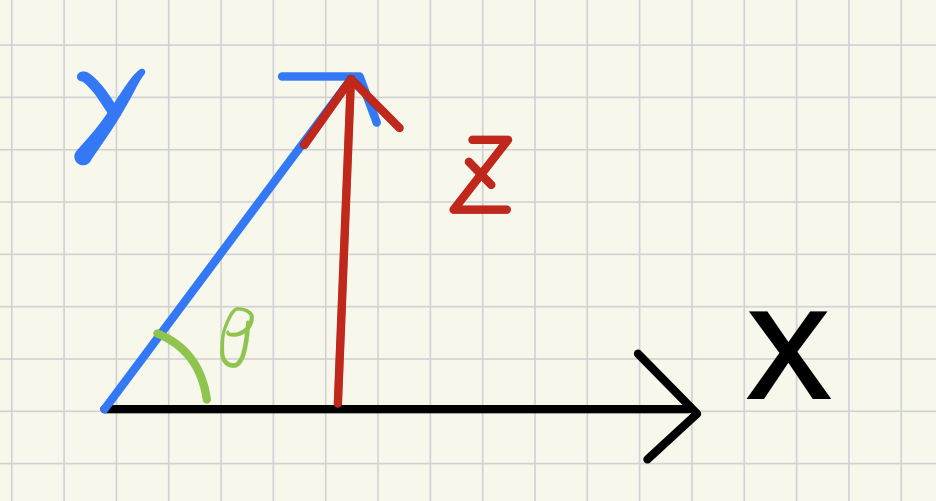
\includegraphics[height=5cm,width=12cm]{CSp.jpeg}
   \end{minipage}
\end{center}
Then all we do rest is just expanding $\abso{y}^2=\abso{z+\tilde{x}}^2$, where $\tilde{x}=y-z=\abso{y}(\cos \theta)\hat{x}$, which give the answer and is easy to compute since $z\cdot \tilde{x}=0$.\\

Now, with Cauchy-Schwarz Inequality, we can check the triangle inequality 
\begin{align*}
  \norm{x+y}^2&=\langle x+y,x+y\rangle \\
&=\langle x,x\rangle +\langle x,y\rangle +\langle y,x\rangle +\langle y,y\rangle \\
&= \langle x,x\rangle + \langle y,y\rangle +2\text{ Re }\langle x,y\rangle \\
&\leq \norm{x}^2 + \norm{y}^2 + 2\abso{\langle x,y\rangle }\\
&\leq \norm{x}^2 + \norm{y}^2 + 2\norm{x}\cdot \norm{y}=\Big(\norm{x}+\norm{y}\Big)^2
\end{align*}
\end{mdframed}
\textbf{(Euclidean Space Abstract Part)} 
\begin{mdframed}
  By a \textbf{concrete Euclidean Space}, we mean some space of $n$-tuple  $(x_1,\dots ,x_n)$ over $\R$, equipped with inner product  $\langle \cdot,\cdot\rangle_E$ defined by 
\begin{align*}
  \langle  (x_1,\dots,x_n)  ,(y_1,\dots ,y_n)\rangle_E= \sqrt{\sum_{k=1}^n (y_k-x_k)^2} 
\end{align*}
By an \textbf{Euclidean Space}, we simply mean a finite dimensional vector space $V$ over $\R$,  equipped with an inner product $\langle \cdot,\cdot\rangle $ such that there exists a concrete Euclidean space $E$ and an isomorphism  $\phi:V\to E$ such that 
\begin{align*}
\hspace{3cm}\langle x,y\rangle= \langle \phi (x),\phi (y)\rangle_E \hspace{1.5cm}(x,y \in V)
\end{align*}
Note that if you define $\langle \cdot,\cdot\rangle $ on the space of $n$-tuples $(x_1,\dots ,x_n)$ over $\R$ by 
\begin{align*}
  \langle  (x_1,\dots,x_n)  ,(y_1,\dots ,y_n)\rangle=2 \sqrt{\sum_{k=1}^n (y_k-x_k)^2} 
\end{align*}
Then, the space of $n$-tuple is clearly not a concrete Euclidean space, and clearly an Euclidean space. 

\end{mdframed}
\textbf{(SVD)}
\section{Operator Norm}
\begin{abstract}
This section introduces the concept of the operator norm and proves some fundamental results related operator norm and finite-dimensional normed spaces. For example, we establish results such as \customref{LOB}{a linear operator being bounded if and only if it is continuous} and \customref{ANoF}{the equivalence of all norms on finite-dimensional vector spaces}.
\end{abstract}
\begin{mdframed}
In this section, and particularly in functional analysis, we say a function $T$ between two metric space is a  \textbf{bounded operator} if $T$ always map bounded set to bounded set. In particular, if $T$ is a linear transformation between two normed space, we say $T$ is a \textbf{bounded linear operator}. Now, suppose $\mathcal{X},\mathcal{Y}$ are two normed space over $\R\text{ or }\C$. In space $L(\mathcal{X},\mathcal{Y})$, alternatively, we can define 
\begin{align*}
T\text{ is bounded } \overset{\triangle}{\iff} \exists M\inr,\forall x\in \mathcal{X}, \norm{Tx}\leq M\norm{x}
\end{align*}
The proof of equivalency is simple. For $(\longrightarrow )$, observe 
\begin{align*}
\norm{Tx}= \norm{x}\cdot\norm{T \frac{x}{\norm{x}}}\leq \Big(\sup \set{\norm{Ty}:\norm{y}=1} \Big)\norm{x}
\end{align*}
For $(\longleftarrow)$, observe 
\begin{align*}
\norm{Tx-Ty}=\norm{T(x-y)}\leq M \norm{x-y}
\end{align*}
We first show that \customref{LOB}{a linear transformation is continuous if and only if it is bounded}. 
\end{mdframed}
\begin{theorem}
\label{LOB}
\textbf{(Liner Operator is Bounded if and only if it is Continuous)} Given two normed space $\mathcal{X},\mathcal{Y}$ over $\R\text{ or }\C$ and  $T\in L(\mathcal{X},\mathcal{Y})$, we have 
\begin{align*}
T\text{ is a bounded operator }\iff T\text{ is continuous on $\mathcal{X}$}
\end{align*}
\end{theorem}
\begin{proof}
If $T$ is bounded, we see that $T$ is Lipschitz. 
\begin{align*}
\norm{Tx-Ty}\leq M \norm{x-y}
\end{align*}
Now, suppose $T$ is linear and continuous at $0$. Let $\epsilon $ satisfy 
\begin{align*}
\sup_{\norm{y}\leq \epsilon } \norm{Ty} \leq 1
\end{align*}
Observe that for all $x \in \mathcal{X}$, we have
\begin{align*}
\norm{Tx}= \frac{\norm{x}}{\epsilon } \bnorm{T \frac{\epsilon x}{\norm{x}}}\leq \frac{\norm{x}}{\epsilon}
\end{align*}
\end{proof}
\begin{mdframed}
Here, we introduce a new terminology, which shall later show its value. Given a set $X$, we say two metrics $d_1,d_2$ on $X$ are \textbf{equivalent}, and write $d_1\sim d_2$, if we have 
\begin{align*}
\exists m,M \inr^+, \forall x ,y\in X, md_1(x,y)\leq d_2(x,y) \leq Md_1(x,y)
\end{align*}
Now, given a fixed vector space $V$, naturally, we say two norms $\norm{\cdot}_1,\norm{\cdot}_2$ on $V$ are \textbf{equivalent} if 
\begin{align*}
\exists m,M \inr^+, \forall x\in X, m \norm{x}_1\leq \norm{x}_2 \leq M\norm{x}_1
\end{align*}
We say two metric $d_1,d_2$ on  $X$ are  \textbf{topologically equivalent} if the topology they induce on $X$ are identical.\\

A few properties can be immediately spotted.  
\begin{enumerate}[label=(\alph*)]
  \item Our definition of $\sim$ between metrics of a fixed $X$ is an equivalence relation.
  \item Our definition of $\sim$ between norms on a fixed $V$ is an equivalence relation.
  \item Equivalent norms induce equivalent metrics.
  \item Equivalent metrics are topologically equivalent. 
\end{enumerate}

We now prove \customref{ANoF}{if $V$ is finite-dimensional, then all norms on  $V$ are equivalent}. This property will later show its value, as used to prove \customref{LmoF}{linear map of finite-dimensional domain is always continuous} 
\end{mdframed}
\begin{theorem}
\label{ANoF}
\textbf{(All Norms on Finite-dimensional space are Equivalent)} Suppose $V$ is a finite-dimensional vector space over $\R\text{ or }\C$. Then 
\begin{align*}
\text{ all norms on $V$ are equivalent }
\end{align*}
\end{theorem}
\begin{proof}
Let $\set{e_1,\dots ,e_n}$ be a basis of $V$. Define $\infty$-norm $\norm{\cdot}_\infty$ on $V$ by 
\begin{align*}
\bnorm{\sum \alpha_i e_i}_{\infty}\triangleq  \max \abso{\alpha_i} 
\end{align*}
It is easily checked that $\norm{\cdot}_\infty$ is indeed a norm. Fix a norm $\norm{\cdot}$ on $V$. We reduce the problem into  
\begin{align*}
  \vi{\text{ finding $m,M\inr^+$ such that }m\norm{x}_\infty \leq \norm{x}\leq M\norm{x}_\infty}
\end{align*}
We first claim 
\begin{align*}
\blue{M=\sum \norm{e_i}\text{ suffices }}
\end{align*}
Compute 
\begin{align*}
\norm{x}= \bnorm{\sum \alpha_ie_i} \leq \sum \abso{\alpha _i} \norm{e_i} \leq \norm{x}_\infty \sum \norm{e_i}= M \norm{x}_\infty \bdone
\end{align*}
Note that reverse triangle inequality give us 
\begin{align}
\label{Lip1}
\Big|\norm{x}-\norm{y}\Big|\leq \norm{x-y} \leq M \norm{x-y}_\infty
\end{align}
Then we can check that 
\begin{enumerate}[label=(\alph*)]
  \item  $\norm{\cdot}:\Big(V,\norm{\cdot}_\infty \Big)\rightarrow \R$ is Lipschitz continuous because of \myref{Equation}{Lip1}.
  \item $S\triangleq \set{y\in V:\norm{y}_\infty=1}$ is sequentially compact in $\norm{\cdot}$ and non-empty. 
\end{enumerate}
Now, by EVT, we know $\min _{y \in S}\norm{y}$ exists. Note that $\min_{y \in S}\norm{y}>0$, since $0 \not\in S$. We claim 
\begin{align*}
  \olive{m= \min_{y \in S}\norm{y}\text{ suffices }}
\end{align*}
Fix $x \in V$ and compute 
\begin{align*}
m\norm{x}_\infty = \norm{x}_\infty (\min_{y \in S} \norm{y})\leq \norm{x}_\infty \cdot  \bnorm{ \frac{x}{\norm{x}_\infty}}=\norm{x}\odone \vdone
\end{align*}






\end{proof}
\begin{theorem}
\label{LmoF}
\textbf{(Linear map of Finite-dimensional Domain is always Continuous)} Given a finite-dimensional normed space $\mathcal{X}$ over $\R\text{ or }\C$, an arbitrary normed space  $\mathcal{Y}$ over $\R\text{ or }\C$ and a linear transformation  $T:\mathcal{X}\rightarrow \mathcal{Y}$, we have 
\begin{align*}
T\text{ is continuous }
\end{align*}
\end{theorem}
\begin{proof}
Fix $x\in \mathcal{X},\epsilon $. We wish 
\begin{align*}
\vi{\text{ to find $\delta$ such that }\forall h\in \mathcal{X}: \norm{h}\leq \delta, \norm{T(x+h)-Tx}\leq \epsilon }
\end{align*}
Let $\set{e_1,\dots ,e_n}$ be a basis of $\mathcal{X}$. Note that $ \norm{ \sum \alpha_i e_i }_1\triangleq  \sum \abso{\alpha _i}$ is a norm. \customref{ANoF}{Because $\mathcal{X}$ is finite-dimensional, we know $\norm{\cdot}$ and $\norm{\cdot}_1$ are equivalent}. Then, we can fix $M\inr^+$ such that 
\begin{align*}
\hspace{2cm}\norm{x}_1 \leq M\norm{x}\hspace{0.5cm}(x \in V)
\end{align*}
We claim 
\begin{align*}
\vi{\delta= \frac{\epsilon }{M(\max \norm{Te_i} )}\text{ suffices }} 
\end{align*}
Fix $\norm{h}\leq \delta$ and express $h=\sum \alpha_i e_i$. Compute using linearity of $T$
\begin{align*}
  \norm{T(x+h)-Tx}&=\norm{\sum \alpha_i T e_i}\\
  &\leq \sum \abso{\alpha _i} \norm{Te_i}\\
  &\leq  \norm{h}_1 (\max \norm{Te_i} )\\
  &\leq M \norm{h}(\max \norm{Te_i})=\epsilon \vdone
\end{align*}
\end{proof}
\begin{mdframed}
We now see that, because \customref{LOB}{Linear transformation is bounded if and only if it is continuous} and \customref{LmoF}{Linear map of finite-dimensional domain is always continuous}, if $\mathcal{X}$ is finite-dimensional, then all linear map of domain $\mathcal{X}$ are bounded. A counter example to the generalization of this statement is followed. 
\begin{Example}{\textbf{(Differentiation is an Unbounded Linear Operator)}}{}
\begin{align*}
\mathcal{X}=\Big(\R[x]|_{[0,1]}, \norm{\cdot}_\infty \Big), D(P)\triangleq P'
\end{align*}
Note that $\set{x^n}_{n\inn}$ is bounded in $\mathcal{X}$ and $\set{D(x^n)}_{n\inn}$ is not.   
\end{Example}
Now, suppose $\mathcal{X},\mathcal{Y}$ are two fixed normed spaces over $\R$ or $\C$. We can easily check that the set $BL(\mathcal{X},\mathcal{Y})$ of bounded linear operators from $\mathcal{X}$ to $\mathcal{Y}$ form a vector space over whichever field $\mathcal{Y}$ is over.\\

Naturally, our definition of boundedness of linear operator derive us a norm on $BL(\mathcal{X},\mathcal{Y})$, as followed 
\begin{align}
\label{tnop}
\norm{T}_{\text{op}}\triangleq \inf \set{M\inr^+ :\forall x \in \mathcal{X}, \norm{Tx}\leq M\norm{x}}
\end{align}
Before we show that our definition is indeed a norm, we first give some equivalent definitions and prove their equivalency. 
\end{mdframed}
\begin{theorem}
\textbf{(Equivalent Definitions of Operator Norm)} Given two fixed normed space $\mathcal{X},\mathcal{Y}$ over $\R$ or  $\C$, a bounded linear operator  $T:\mathcal{X}\rightarrow \mathcal{Y}$, and define $\norm{T}_{\text{op}}$ as in \myref{Equation}{tnop}, we have 
\begin{align*}
\norm{T}_{\text{op}}=\sup_{x\in \mathcal{X},x\neq 0} \frac{\norm{Tx}}{\norm{x}}
\end{align*}
\end{theorem}
\begin{proof}
Define $J\triangleq \set{M\inr^+:\forall x \in \mathcal{X},\norm{Tx}\leq M\norm{x}}$ and observe 
\begin{align*}
J&=\set{M\inr^+:M\geq \frac{\norm{Tx}}{\norm{x}},\forall x\neq 0\in \mathcal{X}}
\end{align*}
This let us conclude 
\begin{align*}
\sup_{x \in \mathcal{X},x\neq 0} \frac{\norm{Tx}}{\norm{x}}=\min  J= \norm{T}_{\text{op}}
\end{align*}
\end{proof}
\begin{mdframed}
It is now easy to see 
\begin{align}
  \norm{T}_{\text{op}}&=\sup_{x \in \mathcal{X},x\neq 0} \frac{\norm{Tx}}{\norm{x}}\label{equivdefopnorm1}\\
&=\sup_{x\in \mathcal{X},\norm{x}=1} \norm{Tx}\label{equivdefopnorm}
\end{align}
It is not all in vain to introduce the equivalent definitions. See that the verification of  $\norm{\cdot}_{\text{op}}$ being a norm on $BL(\mathcal{X},\mathcal{Y})$ become simple by utilizing the equivalent definitions. 
\begin{enumerate}[label=(\alph*)]
  \item For positive-definiteness, fix non-trivial $T$ and fix $x\in \mathcal{X}\setminus N(T)$. Use \myref{Equation}{equivdefopnorm1} to show $\norm{T}_{\text{op}}\geq \frac{\norm{Tx}}{\norm{x}}>0$. 
  \item For absolute homogenity, use \myref{Equation}{equivdefopnorm} and $\norm{Tcx}=\abso{c}\cdot \norm{Tx}$.
  \item For triangle inequality, use \myref{Equation}{equivdefopnorm} and $\norm{(T_1+T_2)x}\leq \norm{T_1x}+\norm{T_2x}$. 
\end{enumerate}
Naturally, and very very importantly, \myref{Equation}{equivdefopnorm1} give us 
\begin{align*}
\hspace{3cm}\norm{Tx}\leq \norm{T}_\text{op}\cdot \norm{x}\hspace{1.5cm}(x\in \mathcal{X})
\end{align*}
This inequality will later be the best tool to help analyze the derivatives of functions between Euclidean spaces, and perhaps better, it immediately give us 
\begin{align*}
 \frac{\norm{T_1T_2x}}{\norm{x}}\leq \frac{\norm{T_1}_\text{op}\cdot \norm{T_2}_\text{op}\cdot \norm{x}}{\norm{x}}=\norm{T_1}_\text{op}\cdot \norm{T_2}_{\text{op}}
\end{align*}
Then \myref{Equation}{equivdefopnorm1} give us  
\begin{align*}
\norm{T_1T_2}_\text{op}\leq \norm{T_1}_\text{op}\cdot \norm{T_2}_\text{op}
\end{align*}
\end{mdframed}
\end{document}
